\chapter[Baryonic Response and Nonlinear Falsification]{Baryonic Response Envelopes and Frozen-Parameter Nonlinear Falsification}
\label{ch:baryonic-response-falsification}

\section{Scope and objective}

The preceding chapters establish a fixed collisionless transfer function, a coupled Einstein--Boltzmann calculation, nonlinear power regeneration, explicit paired halo catalogues, particle-overlap matching, and one-step assembly proxies.  The unresolved interface addressed here is baryonic.  A collisionless halo deficit does not immediately imply a galaxy or satellite deficit because gas retention, photoheating, cooling, star formation, and feedback can amplify or mask the gravitational difference.

This chapter does not pretend to replace hydrodynamics.  It constructs a controlled \emph{response envelope}: the same monotone baryonic map is applied to the cold and refinement halo catalogues over a declared nuisance-parameter family.  This isolates which signatures survive broad common baryonic uncertainty and which remain under-resolved.

The fixed input is the paired $8\,h^{-1}{\rm Mpc}$ halo calculation and its independent $260$- versus $360$-step control.  No refinement parameter is retuned.  The principal result is
\begin{equation}
\boxed{
\begin{gathered}
\text{global baryonic mass budget nearly cold-like},\\
\text{luminous halo count suppressed by roughly }8\%-18\%,\\
\text{near-cutoff matched stellar proxy suppressed much more strongly},\\
\text{CMB and nonlinear lensing remain nearly cold-like},\\
\text{host-centric satellite proxy not yet numerically converged}.
\end{gathered}}
\label{eq:brf-principal-result}
\end{equation}

\section{Declared baryonic response family}

Let $M$ and $V$ denote the halo mass and maximum-circular-speed proxy.  The luminous occupation probability is
\begin{equation}
P_{\rm lum}(V;V_{50},s)
=
\left[1+\exp\left(-\frac{\log(V/V_{50})}{s}\right)\right]^{-1}.
\label{eq:brf-occupation}
\end{equation}
The scan uses
\begin{equation}
V_{50}\in\{15,20,25,30,35,40,50\}\ {\rm km\,s^{-1}},
\qquad
s\in\{0.15,0.25,0.40,0.60\}.
\label{eq:brf-occupation-grid}
\end{equation}

A gas-retention envelope is
\begin{equation}
M_{\rm gas}(M,V)
\propto
\frac{M}{1+(V_{\rm evap}/V)^\eta},
\label{eq:brf-gas-response}
\end{equation}
and a stellar-response proxy is
\begin{equation}
M_\star(M,V)
\propto
\frac{M}{1+(V_{\rm evap}/V)^\eta}
\frac{(V/V_\star)^\alpha}{1+(V/V_\star)^\alpha}.
\label{eq:brf-stellar-response}
\end{equation}
The common response parameters are scanned over
\begin{equation}
\begin{aligned}
V_{\rm evap}&\in\{15,20,25,30,40\}\ {\rm km\,s^{-1}},\\
\eta&\in\{2,3,4,6\},\\
V_\star&\in\{25,40,60,80\}\ {\rm km\,s^{-1}},\\
\alpha&\in\{1,2,3\}.
\end{aligned}
\label{eq:brf-response-grid}
\end{equation}
The cosmic baryon fraction and the maximum conversion efficiency cancel from all refinement-to-cold ratios.  These maps are deliberately broad nuisance envelopes.  They are not calibrated sub-grid physics.

\section{Monotone occupation theorem}

\begin{theorem}[Cumulative ordering implies luminous-count ordering]
Let $\mu_C$ and $\mu_R$ be cold and refinement halo measures on a scalar halo property $x$, with cumulative counts
\[
N_X(>x)=\mu_X((x,\infty)),\qquad X\in\{C,R\}.
\]
Assume
\[
N_R(>x)\le N_C(>x)
\]
for every $x$.  Then every bounded nondecreasing occupation function $p(x)\ge0$ satisfies
\begin{equation}
\int p\,d\mu_R\le\int p\,d\mu_C.
\label{eq:brf-monotone-ordering}
\end{equation}
\end{theorem}

\begin{proof}
For an absolutely continuous $p$ with $p(0)=0$, Stieltjes integration by parts gives
\[
\int p(x)\,d\mu_X(x)
=
\int_0^\infty p'(x)N_X(>x)\,dx.
\]
Since $p'\ge0$, cumulative ordering gives the result.  General bounded nondecreasing $p$ follows by monotone approximation.
\end{proof}

The $360$-step catalogue obeys cumulative refinement-to-cold abundance no greater than one at every archived mass threshold.  The theorem therefore gives a sign-definite luminous-count suppression for any common monotone occupation applied to that time-control catalogue.  The $260$-step catalogue has one isolated high-mass bin slightly above unity because of finite object counts, but every occupation model in the declared scan still yields a total ratio below one.

\section{Global luminous and baryonic envelopes}

The expected luminous count is
\begin{equation}
N_{\rm lum}=\sum_H P_{\rm lum}(V_{\max,H}).
\label{eq:brf-expected-luminous-count}
\end{equation}
The complete occupation scan gives
\begin{center}
\begin{tabular}{lccc}
\toprule
run & minimum & median & maximum\\
\midrule
$260$-step zoom & $0.841250$ & $0.894665$ & $0.920903$\\
$360$-step control & $0.819753$ & $0.874244$ & $0.915456$\\
\bottomrule
\end{tabular}
\end{center}
Thus the global expected luminous-halo count is lower by approximately $8\%-18\%$ throughout the declared occupation family.

\begin{figure}[htbp]
\centering
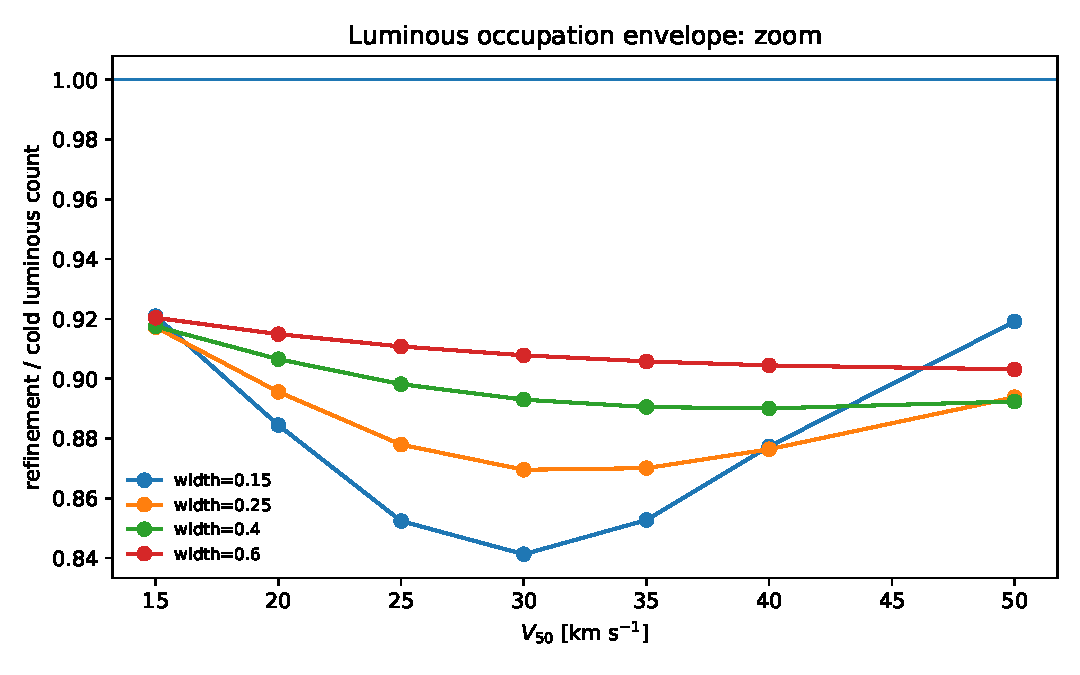
\includegraphics[width=.80\linewidth]{figures/brf/luminous_occupation_zoom.pdf}
\caption{Global luminous-count ratio in the $260$-step zoom catalogue.  Every declared monotone occupation model remains below unity.}
\label{fig:brf-luminous-zoom}
\end{figure}

The integrated baryonic mass budget is much less sensitive because the most massive halos dominate the sum:
\begin{center}
\begin{tabular}{lccc}
\toprule
observable & minimum & median & maximum\\
\midrule
zoom total gas ratio & $0.955236$ & $0.958096$ & $0.963734$\\
zoom total stellar proxy & $0.958112$ & $0.964322$ & $0.968384$\\
time-control total gas ratio & $0.958151$ & $0.961867$ & $0.969067$\\
time-control total stellar proxy & $0.961980$ & $0.970086$ & $0.975786$\\
\bottomrule
\end{tabular}
\end{center}
The model therefore does not predict a comparably large deficit in the total low-redshift baryonic mass budget.  Its sharper signature lies in the distribution of that mass among low-mass objects.

\section{Matched baryonic amplification near the cutoff}

For one matched halo pair, write
\[
R_M=\frac{M_R}{M_C},
\qquad
R_V=\frac{V_R}{V_C}.
\]
For any response of the form
\[
B(M,V)=M f(V)g(V)
\]
with $f$ and $g$ nondecreasing,
\begin{equation}
\frac{B_R}{B_C}
=
R_M\frac{f(R_VV_C)}{f(V_C)}\frac{g(R_VV_C)}{g(V_C)}.
\label{eq:brf-matched-response-ratio}
\end{equation}
Hence
\begin{equation}
R_M\le1,
\quad R_V\le1
\quad\Longrightarrow\quad
\frac{B_R}{B_C}\le R_M\le1.
\label{eq:brf-baryonic-amplification-theorem}
\end{equation}
In the robust zoom sample, $80.303\%$ of matched pairs satisfy both $R_M<1$ and $R_V<1$.

The response scan gives the following median matched stellar-proxy envelopes:
\begin{center}
\small
\begin{tabular}{lccc|ccc}
\toprule
&\multicolumn{3}{c}{260-step zoom}&\multicolumn{3}{c}{360-step control}\\
maximum cold mass & min & median & max & min & median & max\\
\midrule
$3\times10^{10}\,h^{-1}M_\odot$ & $0.1411$ & $0.3962$ & $0.5668$ & $0.1337$ & $0.3881$ & $0.5780$\\
$10^{11}\,h^{-1}M_\odot$ & $0.3371$ & $0.5836$ & $0.6430$ & $0.3128$ & $0.5752$ & $0.6392$\\
$3\times10^{11}\,h^{-1}M_\odot$ & $0.6266$ & $0.7130$ & $0.7468$ & $0.5941$ & $0.6997$ & $0.7424$\\
$10^{12}\,h^{-1}M_\odot$ & $0.7157$ & $0.7627$ & $0.7827$ & $0.7092$ & $0.7457$ & $0.7817$\\
\bottomrule
\end{tabular}
\end{center}

\begin{figure}[htbp]
\centering
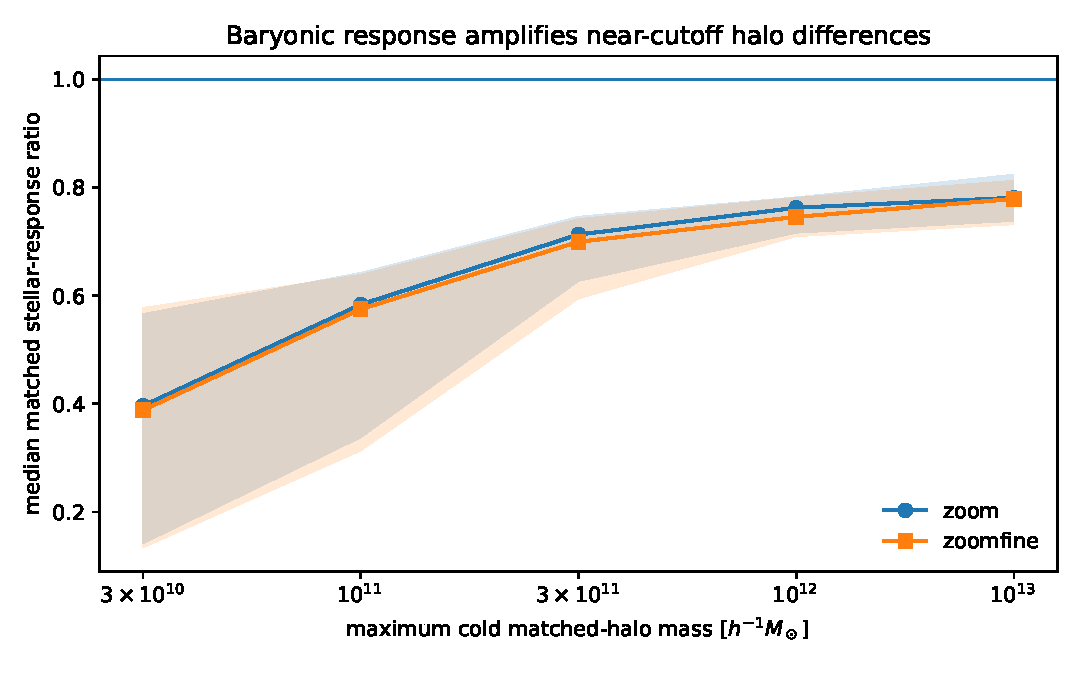
\includegraphics[width=.82\linewidth]{figures/brf/matched_stellar_response_envelope.pdf}
\caption{The same baryonic response applied to matched halos amplifies the gravitational difference near the cutoff.  Shaded regions show the full declared response envelope.}
\label{fig:brf-matched-stellar}
\end{figure}

For matched halos below $3\times10^{10}\,h^{-1}M_\odot$, the median stellar proxy is only about $0.39$ of the cold value.  The time-control discrepancy in that median is $0.00805$.  The near-cutoff conclusion is therefore materially stronger and more stable than the small difference in the total stellar budget.

\section{Structural and lensing proxies}

The matched catalogue directly supplies mass, half-mass radius, $V_{\max}$, and velocity-dispersion proxies.  Define
\begin{equation}
\Sigma_{1/2}^{\rm proxy}
:=
\frac{M}{2\pi r_{1/2}^2},
\qquad
S_{\rm dyn}^{\rm proxy}
:=
\frac{V_{\max}^2}{r_{1/2}}.
\label{eq:brf-structural-proxies}
\end{equation}
Their refinement-to-cold ratios are
\begin{equation}
R_{\Sigma}
=
\frac{R_M}{R_{r_{1/2}}^2},
\qquad
R_{\rm dyn}
=
\frac{R_V^2}{R_{r_{1/2}}}.
\label{eq:brf-structural-ratios}
\end{equation}
For the robust zoom sample,
\begin{equation}
\boxed{
\operatorname{median}R_{\Sigma}=0.925269,
\qquad
\operatorname{median}R_{\rm dyn}=0.933888.
}
\label{eq:brf-structural-medians}
\end{equation}
The fractions below unity are $0.681818$ and $0.696970$, respectively.

\begin{figure}[htbp]
\centering
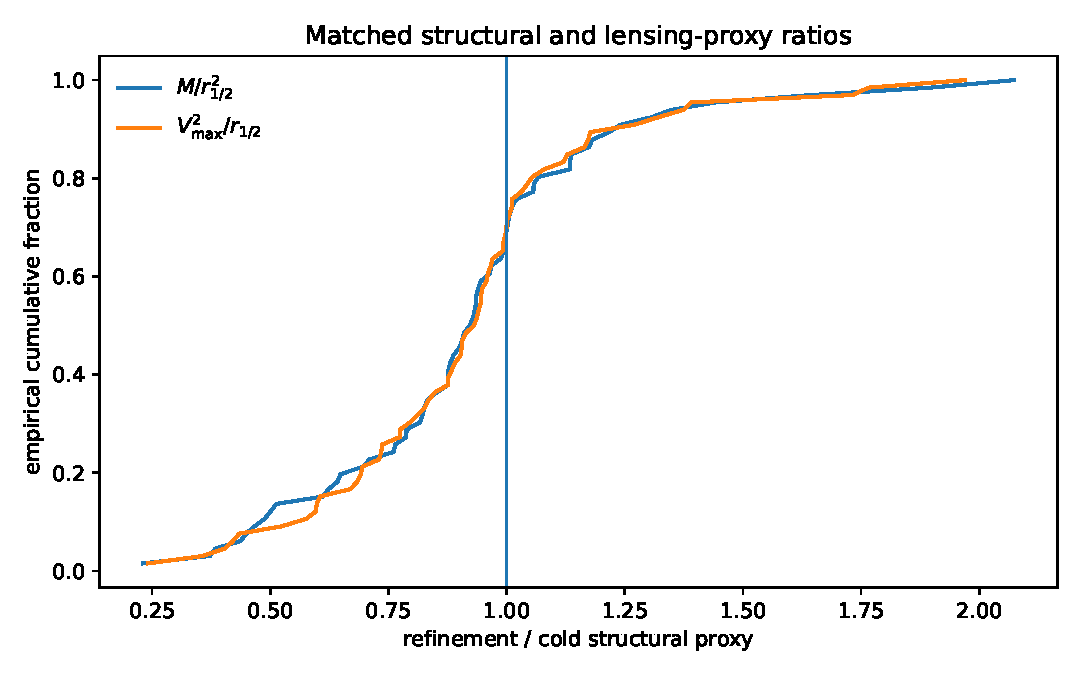
\includegraphics[width=.80\linewidth]{figures/brf/matched_surface_density_cdf.pdf}
\caption{Empirical cumulative distributions of the matched half-mass and dynamical surface-density proxies.}
\label{fig:brf-surface-cdf}
\end{figure}

These are not precision galaxy--galaxy lensing predictions because the FoF mass is not a calibrated spherical-overdensity mass and no resolved baryonic profile is present.  They do show that the matched near-cutoff structures tend to have lower projected and dynamical density scales before any branch-dependent baryonic compensation is introduced.

\section{Frozen-parameter cross-observable signature}

For any observable ratio $R<1$, define the branch-dependent baryonic enhancement required to restore unity,
\begin{equation}
\Delta_B^{\rm erase}:=\frac1R-1.
\label{eq:brf-erasure-boost}
\end{equation}
This does not assert whether such a boost is astrophysically plausible.  It states the exact differential response required to erase the gravitational prediction.

\begin{center}
\small
\begin{tabular}{p{.47\linewidth}rr}
\toprule
observable & $R$ & required boost\\
\midrule
CMB lensing at $L=3000$ & $0.995081$ & $0.49\%$\\
nonlinear galaxy lensing, $z_s=0.5$, $\ell=5000$ & $0.985017$ & $1.52\%$\\
global luminous count, zoom median & $0.894665$ & $11.77\%$\\
global luminous count, time control & $0.874244$ & $14.38\%$\\
matched stellar proxy, $M\le3\times10^{10}\,h^{-1}M_\odot$ & $0.396164$ & $152.42\%$\\
matched half-mass surface-density proxy & $0.925269$ & $8.08\%$\\
atomic-cooling collapsed fraction at $z=7.4$ & $0.342283$ & $192.16\%$\\
\bottomrule
\end{tabular}
\end{center}

\begin{figure}[htbp]
\centering
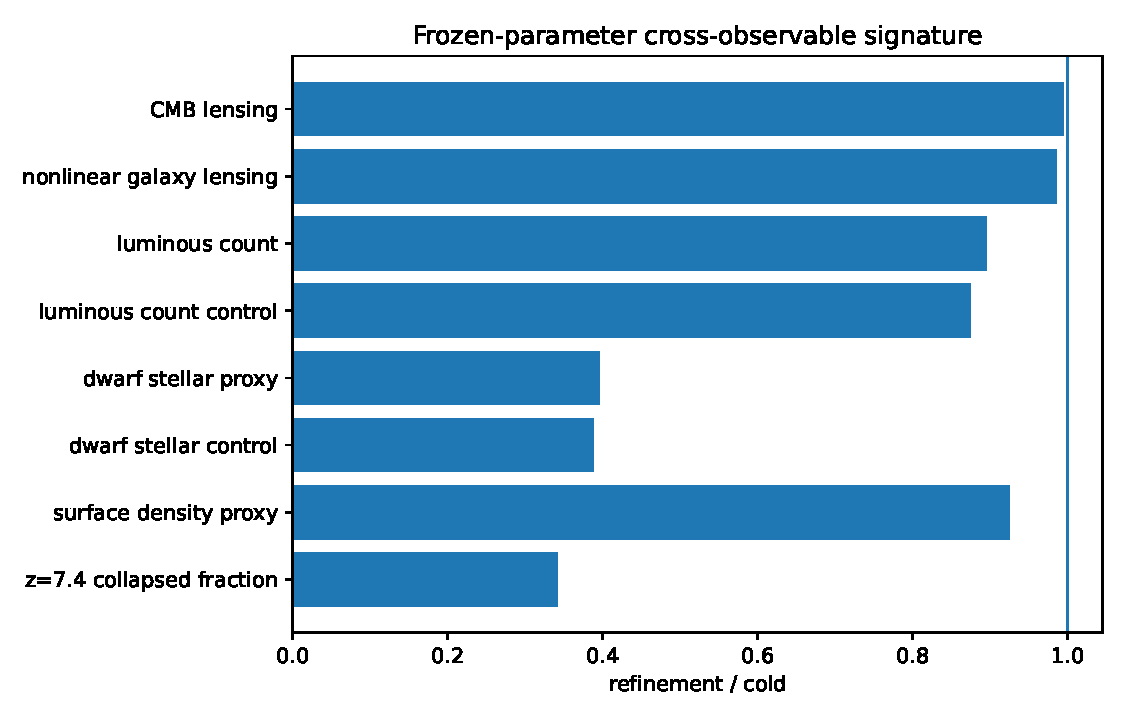
\includegraphics[width=.84\linewidth]{figures/brf/joint_falsification_signature.pdf}
\caption{One frozen dark-sector parameter set predicts nearly cold CMB and nonlinear lensing together with much stronger dwarf-scale and high-redshift suppression.}
\label{fig:brf-joint-signature}
\end{figure}

The cross-observable pattern is therefore
\begin{equation}
\boxed{
\text{CMB and bulk lensing nearly cold}
\quad+
\text{dwarf luminosity and early collapse strongly suppressed}.
}
\label{eq:brf-linked-signature}
\end{equation}
A data set showing the opposite combination would reject this branch more sharply than any one observable alone.

\section{Satellite-neighborhood negative control}

A host-centric count was also constructed around the five most massive matched hosts.  Every neighboring FoF halo within radius $R$ was weighted by the same occupation family.  This is only a satellite-candidate proxy because the FoF catalogue does not resolve subhalos inside the host component.

\begin{center}
\begin{tabular}{lcccc}
\toprule
run & $R\,[h^{-1}{\rm Mpc}]$ & minimum & median & maximum\\
\midrule
zoom & $0.5$ & $0.825$ & $1.283$ & $1.344$\\
zoom & $1.0$ & $0.985$ & $1.156$ & $1.223$\\
zoom & $1.5$ & $0.934$ & $1.052$ & $1.112$\\
time control & $0.5$ & $0.403$ & $1.039$ & $1.102$\\
time control & $1.0$ & $0.915$ & $1.009$ & $1.070$\\
time control & $1.5$ & $0.900$ & $0.976$ & $1.020$\\
\bottomrule
\end{tabular}
\end{center}

\begin{figure}[htbp]
\centering
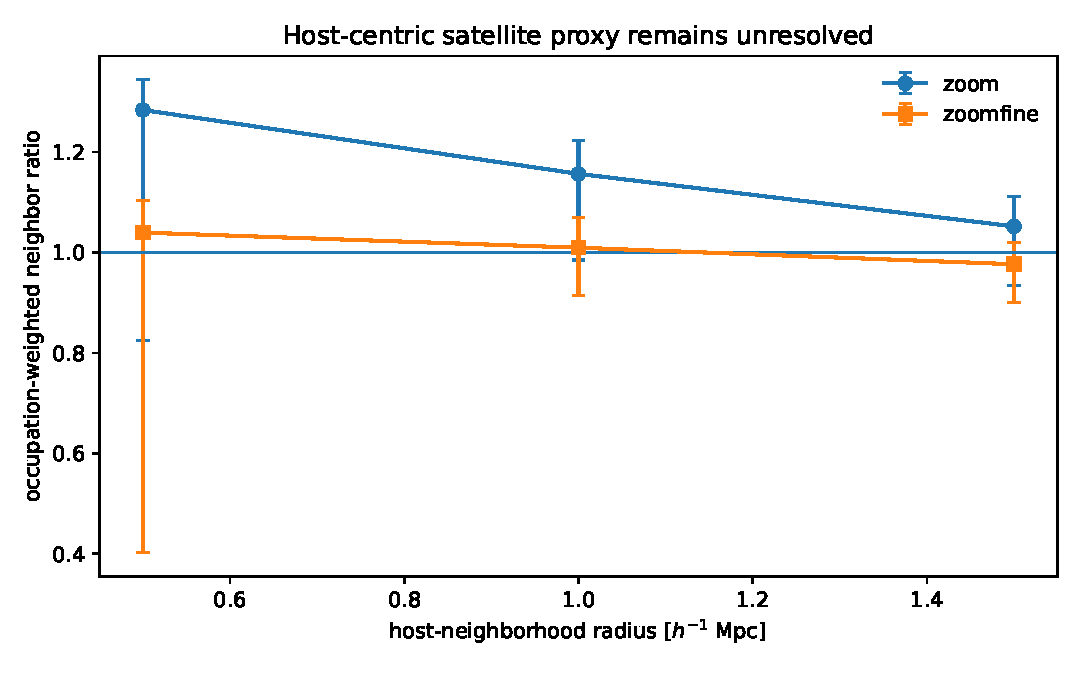
\includegraphics[width=.80\linewidth]{figures/brf/host_neighborhood_control.pdf}
\caption{The host-neighborhood proxy changes materially under the time-step control and crosses unity across the baryonic envelope.  It is not yet a stable satellite prediction.}
\label{fig:brf-host-control}
\end{figure}

This negative control is important.  The global luminous count and matched dwarf response are stable, but a true satellite prediction requires a subhalo finder, higher force resolution, host zooms, and disruption tracking.

\section{Verification ledger}

The deterministic audit records
\begin{equation}
\boxed{20\ {\rm PASS},\qquad0\ {\rm FAIL}.}
\label{eq:brf-pass-count}
\end{equation}
Selected controls are
\begin{center}
\begin{tabular}{lr}
\toprule
control & residual or value\\
\midrule
maximum global occupation ratio & $0.920903$\\
zoom/time-control occupation-median difference & $0.020421$\\
near-cutoff response-median difference & $0.008050$\\
median half-mass surface-density ratio & $0.925269$\\
robust matches with both $M_R<M_C$ and $V_R<V_C$ & $0.803030$\\
CMB-lensing ratio at $L=3000$ & $0.995081$\\
nonlinear galaxy-lensing ratio at $\ell=5000$ & $0.985017$\\
reionization efficiency penalty at $z=7.4$ & $2.921558$\\
\bottomrule
\end{tabular}
\end{center}
The input hashes, full response scans, structural tables, and check records are included in the reproducibility package.

\section{Claim boundary}

This chapter establishes:
\begin{itemize}
\item an exact monotone occupation-ordering theorem;
\item a frozen common-response envelope for luminous counts, gas, and stellar proxies;
\item a matched-halo theorem showing how velocity suppression amplifies baryonic suppression;
\item controlled near-cutoff stellar-response and structural-proxy ratios;
\item a cross-observable erasure threshold with no dark-sector retuning;
\item a negative control showing that the present host-centric satellite proxy is not converged.
\end{itemize}

It does not establish:
\begin{itemize}
\item hydrodynamic cooling, star formation, or feedback from first principles;
\item resolved subhalo catalogues or disruption histories;
\item calibrated galaxy luminosities or stellar-mass functions;
\item survey selection, covariance, foregrounds, or a likelihood;
\item microscopic values of $a_\star$, $\Lambda$, $\gamma$, or the physical mass scale;
\item radiative stability, independent reproduction, or literature priority.
\end{itemize}

